\documentclass{article}
\usepackage{graphicx} % Required for inserting images
\usepackage[margin=2.5cm]{geometry}
\usepackage[T1]{fontenc}
\usepackage{lmodern}
\usepackage{amsmath}
\usepackage{booktabs}
\usepackage{caption}
\usepackage[numbers,sort&compress]{natbib}
\usepackage[hidelinks]{hyperref}

\graphicspath{{figures/}{./}}

\title{HealthMonitoring}
\author{Manideepa Mukherjee Bhakat}
\date{October 2026}

\begin{document}
\maketitle

\begin{center}
{\Large\textbf{BodySync: A Personal-Normal Score from Wrist Physiology, Tested on Eight Empatica Datasets}}
\end{center}

\begin{abstract}
Wrist wearables record heart rate, electrodermal activity (EDA) and skin temperature continuously, but turning these signals into a meaningful everyday score remains difficult. We compared two candidate scores on the same data. Score~A (\emph{sync}) measures whether the three signals move together the way they usually do for a person. Score~B (\emph{BodySync}) measures how far their levels are from the person's own normal for the same situation, counting only changes in the stress direction. Both were built on ZU-PWD~'25, a free-living Empatica EmbracePlus dataset (27 people, 901{,}440 minutes), and evaluated on seven public Empatica E4 stress datasets. Coupling features were close to chance at telling sleep, rest and activity apart (balanced accuracy 0.37 vs.\ 0.81 for signal levels). Across the stress datasets the sync score did not separate stress from calm in any fair test (within-person AUC 0.46--0.52). BodySync separated acute laboratory stress on WESAD (AUC 0.78, 12 of 15 people) and weakly on a second laboratory dataset (AUC 0.60), but was at chance on all three everyday-life datasets. Signal levels relative to a personal normal therefore carry more information than signal coupling. Neither score detects everyday stress from one-minute or five-minute wrist summaries.
\end{abstract}

\section{Introduction}

Sun et al.~\cite{sun2026trust} showed that EDA, heart-rate variability and skin temperature change when people read health information, and predicted trust from these signals. Their signals were analysed separately, in a single laboratory session, and the authors call for longitudinal, ecological studies. Our starting idea (\emph{BodySync}) was to look at the relationships between signals instead: when the body is in a familiar state its signals should move together in a familiar way, and a break in that pattern (a \emph{desync}) might mark stress, illness or poor sleep. Network physiology supports the idea that coupling between organ systems changes with state~\cite{bashan2012network}, and coupling features have improved emotion recognition in the laboratory~\cite{valenza2013coupling}.

The dataset we started from, ZU-PWD~'25~\cite{evangelista2025zupwd}, already has a wellness score: the Physiological Wellness Index~\cite{sharma2025pwi}, a hand-weighted average of signal levels. It was checked on a few example days only, and the free copy of the dataset has no stress labels. We therefore set out to (i) test whether coupling adds information over signal levels on ZU-PWD, (ii) build two candidate scores, sync (A) and a personal-normal score (B), and (iii) test both on every public Empatica dataset with stress labels we could obtain.

\section{Data}

\paragraph{ZU-PWD~'25.} Twenty-seven people wore an Empatica EmbracePlus in daily life between March 2024 and May 2025. The free copy has 901{,}440 one-minute rows with 24 columns, including pulse rate, EDA, skin temperature, sleep stage and activity intensity. After removing minutes when the watch was not worn (wear detection $<$50\%) and implausible values (heart rate outside 35--200~bpm, temperature outside 25--40\,$^\circ$C), 484{,}636 minutes had all three signals. Each minute was labelled \emph{asleep} (sleep stage 101), \emph{resting} (awake and sedentary), \emph{active} (awake, moderate or vigorous activity) or \emph{other}. These labels come from Empatica's own accelerometer-based algorithms. Heart-rate variability and breathing rate are mostly recorded only when the wrist is still, so we used heart rate, EDA and temperature.

\paragraph{External datasets.} Table~\ref{tab:datasets} lists the seven public Empatica E4 datasets with stress labels. The E4 is the predecessor of the EmbracePlus and records the same three signals at a higher rate. Each dataset was converted to a common window format: 2-minute windows sliding by 30~s for the laboratory protocols, and 5-minute windows for everyday-life data.

\begin{table}[htbp]
\centering
\caption{Public Empatica E4 datasets used for validation. Citations from OpenAlex, October 2026.}
\label{tab:datasets}
\footnotesize
\begin{tabular}{llrlrl}
\toprule
Dataset & Paper & Cites & Setting & People & Stress label \\
\midrule
WESAD & Schmidt 2018~\cite{schmidt2018wesad} & 1{,}352 & lab & 15 & Trier Social Stress Test \\
Nurse stress & Hosseini 2022~\cite{hosseini2022nurse} & 119 & hospital & 15 & nurse-rated stress \\
Stress-Predict & Iqbal 2022~\cite{iqbal2022stresspredict} & 113 & lab & 35 & Stroop test, interview \\
Stress + exercise & Hongn 2025~\cite{hongn2025stress} & 37 & lab & 36 & arithmetic/emotional tasks \\
EmpaticaE4Stress & Campanella 2024~\cite{campanella2024e4stress} & 26 & lab & 29 & timed puzzle tasks \\
ADARP & Sah 2022~\cite{sah2022adarp} & 13 & daily life & 11 & button press when stressed \\
CAN-STRESS & Rahimi Azghan 2025~\cite{azghan2025canstress} & 1 & daily life & 62 & stress ratings 0--9 \\
\bottomrule
\end{tabular}
\end{table}

\begin{figure}[htbp]
\centering
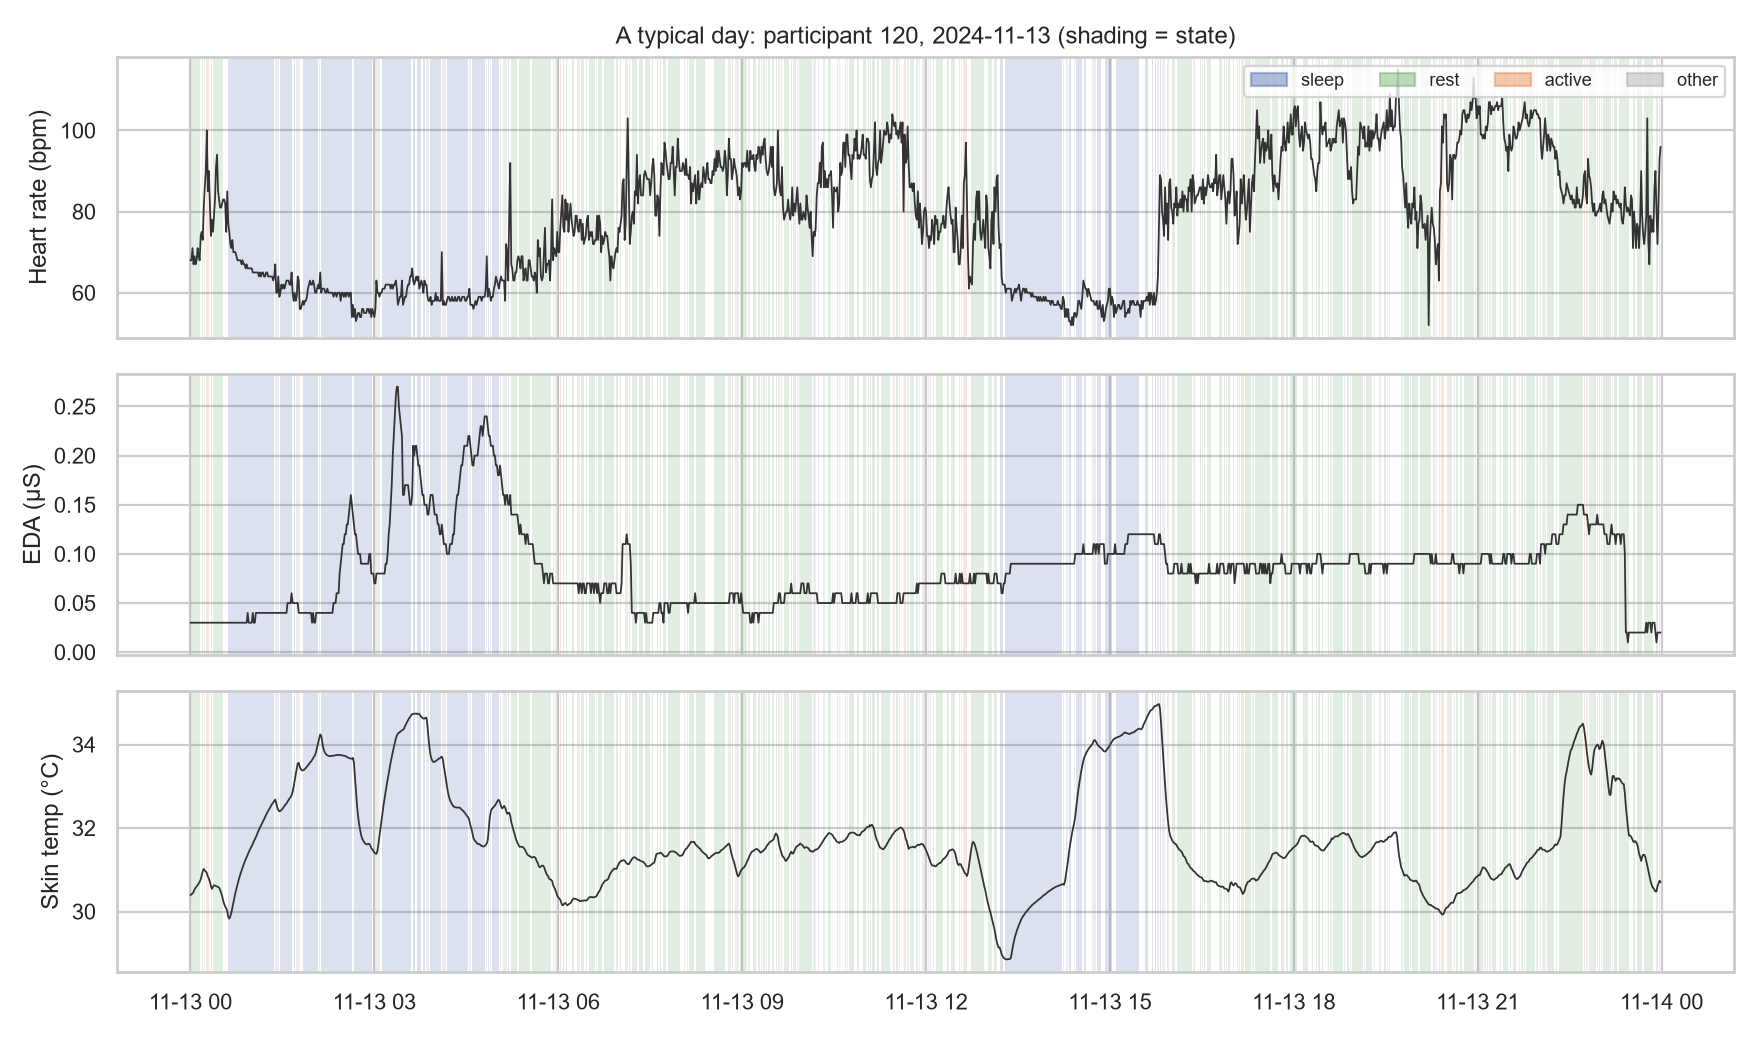
\includegraphics[width=0.95\linewidth]{fig1_typical_day.png}
\caption{One day of ZU-PWD data for one participant. Shading shows the watch's state label.}
\label{fig:day}
\end{figure}

\section{Methods}

\subsection{Windows and features (ZU-PWD)}
Each person's timeline was cut into 30-minute windows sliding by 15 minutes. A window was given a state only if at least 70\% of its minutes shared it; otherwise it was \emph{other}. Windows needed at least 75\% of minutes with all three signals. \emph{Level} features were the mean and standard deviation of each signal. \emph{Personal} features were each mean relative to the person's own median and interquartile range. \emph{Coupling} features were the Pearson correlation of each signal pair (HR--EDA, HR--temperature, EDA--temperature), on raw values and on minute-to-minute changes.

\subsection{Does coupling add information?}
XGBoost classified windows as sleep, rest or active, and separately sleep vs.\ rest (both still, so movement cannot separate them). Each person was tested on a model trained on the others (leave-one-subject-out). Per-person balanced accuracy was compared between feature sets with a paired Wilcoxon test.

\subsection{The two scores}
Both scores use the same steps on different inputs:
\begin{enumerate}
\item For each person and situation, the \emph{normal} is the median of each input across that person's windows in that situation, and the typical spread is the scaled median absolute deviation. Situations with fewer than 10 windows fall back to the person's overall normal.
\item Each input becomes a number of typical spreads away from normal, $z$; the distance is the root mean square of the $z$ values.
\item The score is $100 / (1 + d/2)$, so the normal scores 100 and two spreads away scores 50.
\end{enumerate}
\textbf{Score A (sync)} uses the three pairwise correlations as inputs, and any deviation counts. \textbf{Score B (BodySync)} uses mean heart rate, log EDA and mean skin temperature, and only deviations in the stress direction count (heart rate up, EDA up, temperature down). The input furthest from normal is reported as the reason for a low score.

\paragraph{Situations and normals.} In ZU-PWD the situation is the watch's state label, and all windows define the normal. In the external everyday-life datasets, which have no sleep labels, windows were split into still and moving at each person's median movement. In the laboratory datasets the normal is the baseline rest period.

\subsection{Evaluation}
For each dataset and score we report the within-person AUC: how well a lower score separates a person's stress windows from their calm windows, averaged over people (0.5 = chance). We also report how many people scored lower under stress, with a paired Wilcoxon test. To avoid an unfair advantage, laboratory stress was compared with \emph{later} rest, amusement or meditation, never with the baseline that set the normal. EmpaticaE4Stress has no later rest, so it is the one exception and is marked as a weaker test. In the nurse data the stress intervals were first selected by the authors' EDA-based detector. We therefore compared flagged intervals the nurse rated as stressful with flagged intervals rated as not stressful.

\section{Results}

\subsection{Coupling vs.\ levels on ZU-PWD}
Coupling features alone were close to chance (Table~\ref{tab:coupling}). Adding them to level and personal features raised balanced accuracy by less than one percentage point. That gain was detectable for the three-class task but not for sleep vs.\ rest (Table~\ref{tab:coupling_paired}). The correlations themselves overlapped almost completely across states (Figure~\ref{fig:coupling}).

\begin{table}[htbp]
\centering
\caption{Leave-one-subject-out balanced accuracy on ZU-PWD (chance: 0.33 and 0.50).}
\label{tab:coupling}
\begin{tabular}{lcc}
\toprule
Features & Sleep / rest / active & Sleep vs rest \\
\midrule
Coupling only & 0.372 & 0.562 \\
Levels & 0.807 & 0.831 \\
Levels + personal & 0.825 & 0.878 \\
Levels + personal + coupling & 0.835 & 0.884 \\
\bottomrule
\end{tabular}

\end{table}

\begin{table}[htbp]
\centering
\caption{Per-person paired comparisons (Wilcoxon signed-rank test).}
\label{tab:coupling_paired}
\small
\begin{tabular}{llccc}
\toprule
Task & Comparison & Median gain & People better & $p$ \\
\midrule
Sleep / rest / active & levels + personal + coupling vs levels + personal & +0.006 & 13/20 & 0.006 \\
Sleep / rest / active & coupling only vs levels & -0.397 & 0/20 & $<$0.001 \\
Sleep vs rest & levels + personal + coupling vs levels + personal & +0.003 & 10/18 & 0.326 \\
Sleep vs rest & coupling only vs levels & -0.286 & 0/18 & $<$0.001 \\
\bottomrule
\end{tabular}

\end{table}

\begin{figure}[htbp]
\centering
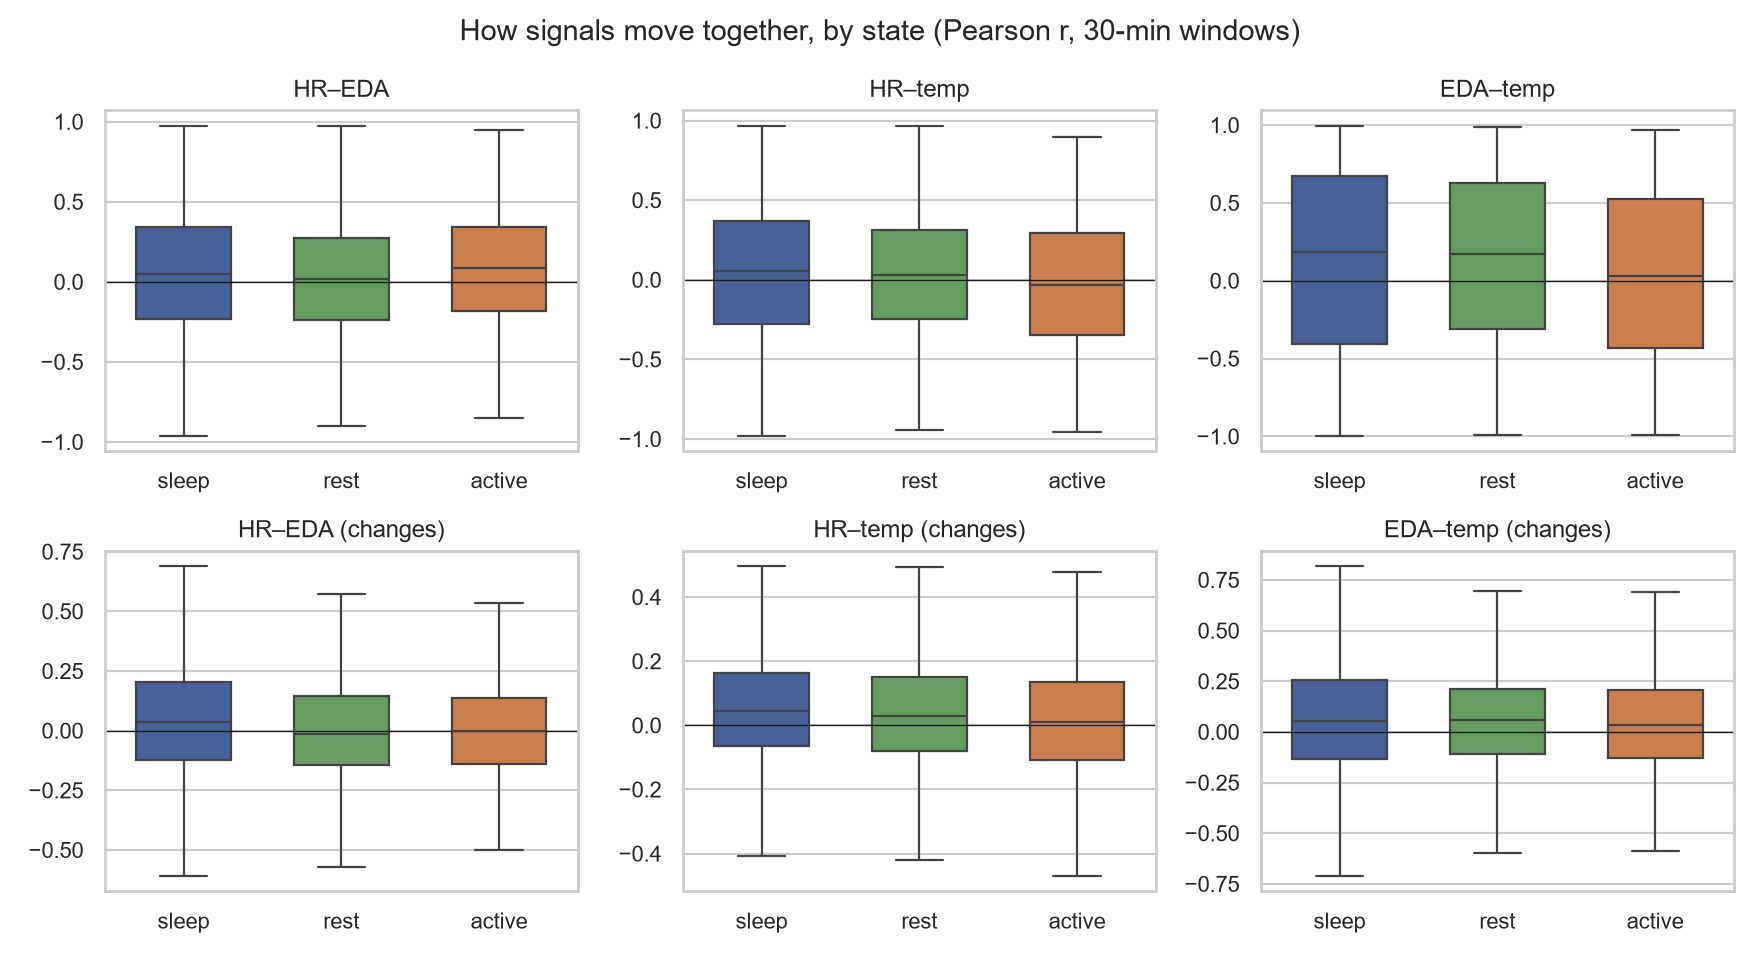
\includegraphics[width=0.85\linewidth]{fig2_coupling_by_state.png}
\caption{Pairwise correlations in 30-minute windows by state. The distributions overlap almost completely.}
\label{fig:coupling}
\end{figure}

\subsection{The scores on ZU-PWD}
With situation-aware normals, active windows scored like the other situations. With one normal for everything, activity looked like stress (Table~\ref{tab:exercise_zupwd}). Neither score was lower on days after nights with more wake-ups, more time awake or less sleep (Table~\ref{tab:sleep}). Figure~\ref{fig:week} shows a week of BodySync scores for one participant.

\begin{table}[htbp]
\centering
\caption{Median BodySync score by situation on ZU-PWD.}
\label{tab:exercise_zupwd}
\begin{tabular}{lcc}
\toprule
Situation & Situation-aware normal & One normal for all \\
\midrule
Sleep & 75.6 & 91.1 \\
Rest & 79.2 & 81.6 \\
Active & 78.6 & 62.8 \\
Other & 78.1 & 75.0 \\
\bottomrule
\end{tabular}

\end{table}

\begin{table}[htbp]
\centering
\caption{Next-day (08:00--22:00) mean score after each person's worse vs.\ better nights.}
\label{tab:sleep}
\small
\begin{tabular}{llcccc}
\toprule
Score & Bad night = & After bad & After good & People lower & $p$ \\
\midrule
A (sync) & More wake-ups & 71.6 & 71.6 & 6/12 & 0.850 \\
A (sync) & More time awake & 71.5 & 71.7 & 8/12 & 0.519 \\
A (sync) & Less sleep & 71.4 & 71.7 & 7/12 & 0.622 \\
B (BodySync) & More wake-ups & 76.5 & 76.4 & 7/12 & 0.970 \\
B (BodySync) & More time awake & 75.8 & 77.1 & 8/12 & 0.424 \\
B (BodySync) & Less sleep & 76.8 & 76.4 & 6/12 & 0.791 \\
\bottomrule
\end{tabular}

\end{table}

\begin{figure}[htbp]
\centering
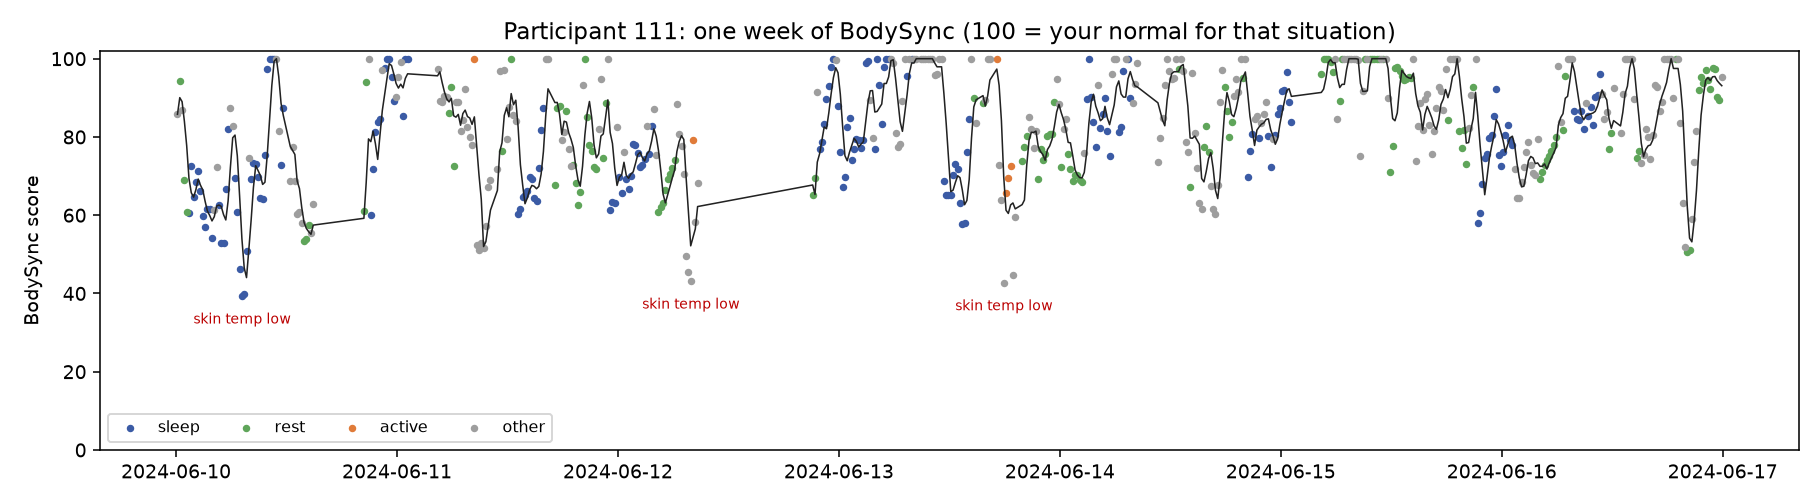
\includegraphics[width=\linewidth]{fig3_example_week.png}
\caption{One week of BodySync scores for one participant, with the reason given for the three lowest points.}
\label{fig:week}
\end{figure}

\subsection{Sync vs.\ BodySync on the stress datasets}
Table~\ref{tab:results} and Figure~\ref{fig:avb} show the main comparison. On every fair test the sync score was at chance (AUC 0.46--0.52), including on WESAD. BodySync separated stress clearly on WESAD (AUC 0.78; lower under stress for 12 of 15 people) and weakly on the stress + exercise dataset (AUC 0.60). It was at chance on Stress-Predict and on all three everyday-life datasets. Both scores were high on EmpaticaE4Stress, but that test compares stress with the baseline that defined the normal, so it overstates performance. When BodySync dropped under stress, the most common reason given was high EDA.

\begin{table}[htbp]
\centering
\caption{Stress vs.\ calm for both scores. AUC: within-person AUC averaged over people. Lower: people whose mean score was lower under stress. Bold: the higher AUC of the two scores. $^\dagger$Weaker test (stress vs.\ the baseline that set the normal).}
\label{tab:results}
\resizebox{\linewidth}{!}{\begin{tabular}{llccccccc}
\toprule
 & & & \multicolumn{3}{c}{A: sync} & \multicolumn{3}{c}{B: BodySync} \\
\cmidrule(lr){4-6}\cmidrule(lr){7-9}
Dataset & Setting & $n$ & AUC & Lower & $p$ & AUC & Lower & $p$ \\
\midrule
WESAD & lab & 15 & 0.46 & 6/15 & 0.359 & \textbf{0.78} & 12/15 & 0.004 \\
Nurse stress & free-living & 11 & \textbf{0.52} & 5/11 & 0.577 & 0.52 & 7/11 & 0.765 \\
Stress-Predict & lab & 35 & 0.48 & 15/35 & 0.501 & \textbf{0.54} & 19/35 & 0.342 \\
Stress + exercise & lab & 35 & 0.49 & 16/35 & 0.554 & \textbf{0.60} & 21/35 & 0.016 \\
EmpaticaE4Stress$^\dagger$ & lab & 29 & 0.90 & 29/29 & $<$0.001 & \textbf{0.92} & 28/29 & $<$0.001 \\
ADARP & free-living & 11 & \textbf{0.48} & 4/11 & 0.123 & 0.45 & 4/11 & 0.240 \\
CAN-STRESS & free-living & 27 & 0.52 & 16/27 & 0.400 & \textbf{0.54} & 18/27 & 0.485 \\
\bottomrule
\end{tabular}
}
\end{table}

\begin{figure}[htbp]
\centering
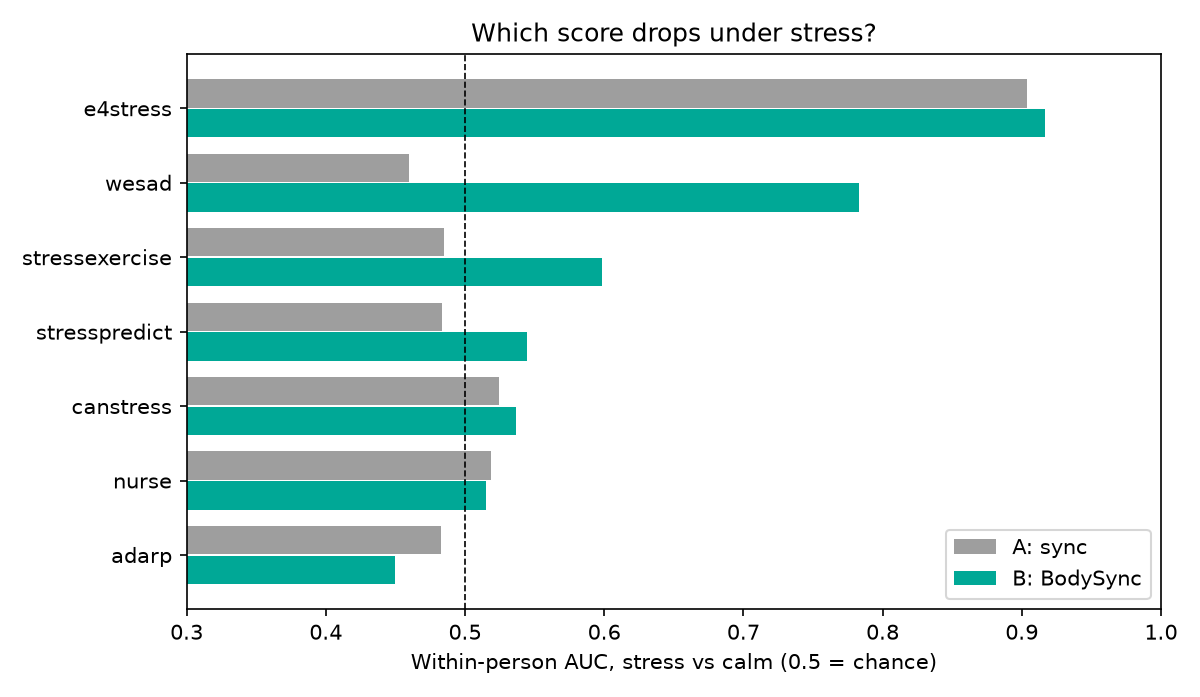
\includegraphics[width=0.75\linewidth]{fig5_sync_vs_bodysync.png}
\caption{Within-person AUC of both scores on each dataset. The dashed line marks chance.}
\label{fig:avb}
\end{figure}

\paragraph{Exercise.} In the stress + exercise dataset, cycling scored lower than the stress tasks on both scores (Table~\ref{tab:exercise}). The laboratory sessions have no ``exercising normal'' to compare against, unlike ZU-PWD, so a workout looks like a strong deviation.

\begin{table}[htbp]
\centering
\caption{Median score by condition in the stress + exercise dataset.}
\label{tab:exercise}
\begin{tabular}{lcc}
\toprule
Condition & A: sync & B: BodySync \\
\midrule
Baseline & 72.3 & 83.7 \\
Rest & 55.5 & 60.6 \\
Stress & 46.8 & 44.5 \\
Aerobic & 36.8 & 16.8 \\
Anaerobic & 48.0 & 17.4 \\
Recovery & 53.1 & 26.9 \\
\bottomrule
\end{tabular}

\end{table}

\section{Discussion}

The original BodySync idea, that a break in how signals move together marks stress, was not supported. Coupling barely differed between sleep, rest and activity in free-living data, and the sync score was at chance on every fair stress test. This agrees with Xu et al.~\cite{xu2026pilot}, who found that correlation features from consumer wearables did not beat EDA alone. Laboratory work that found coupling useful used ECG and respiration belts at much higher resolution~\cite{valenza2013coupling}. We found no benefit even on WESAD at one sample per second, so the problem is not only ZU-PWD's one-minute resolution.

Signal levels compared with a personal normal carried most of the information. BodySync picked up the strong, acute response to the Trier Social Stress Test, mainly through rising EDA. Situation-aware normals kept exercise from looking like stress in ZU-PWD, a known weakness of context-free wrist stress detection~\cite{gjoreski2017context}. Personal baselines are also the basis of wearable illness detection~\cite{mishra2020presymptomatic}.

The everyday-life results show the main limit. In ADARP, CAN-STRESS and the nurse data, average heart rate, EDA and temperature were nearly identical in moments people reported as stressful and in calm ones. Self-reports are sparse and imprecise in time, but the same pattern held across three independent datasets. Wrist stress models are known to generalise poorly beyond the dataset they were built on, and our results are consistent with that.

\paragraph{Limitations.}
\begin{itemize}
\item \textbf{Retrospective normal:} each person's normal is computed from their whole recording, including later data. A deployed version needs a calibration period or a past-only, rolling normal.
\item \textbf{No drift handling:} the normal is fixed, so slow changes (over weeks, or within a laboratory session) are not adjusted for.
\item \textbf{State labels:} ZU-PWD states come from Empatica's algorithms, not ground truth. The free copy has no stress labels, so stress could only be tested on the E4 datasets.
\item \textbf{Sample:} several datasets are small (11--15 people), and two ZU-PWD participants hold about half the data.
\end{itemize}

\section{Conclusion}

We compared a coupling-based sync score with a personal-normal score, BodySync, on one free-living EmbracePlus dataset and seven public E4 stress datasets. How signals move together added almost nothing. How far their levels are from a person's own normal detected acute laboratory stress on the field's standard benchmark. Neither score detected everyday stress. BodySync is best described as a measure of how different the body is from its usual state: it captures strong physiological responses, but it is not a validated everyday stress detector.

\paragraph{Code and data.} Code, result tables and figures: \url{https://github.com/swaylakh/bodysync}. Dataset sources are listed in the repository README.

\bibliographystyle{unsrtnat}
\bibliography{refs}

\end{document}
